% !TEX root = ../thesis.tex
%

{\usekomafont{chapter}Résumé}
\label{cha:abstract-diff} \\


La contribution principale de cette thèse est la conception de la plateforme robotique Poppy qui peut avoir des applications dans les domaines scientifiques, artistiques et pédagogiques. Poppy est une plate-frome robotique communautaire, modulaire et reproductible.

Dans ce manuscrit sera introduit le context et les challenges scientifiques qui ont motivé la conception d'une nouvelle platforme. Ensuite nous presentrons notre approche de conception ouvrant la possibilité de librement modifier la morphologie d'un robot tout en assurant d'assurer sa reproductibilité scientifique. Puis nous décrirons la plate-forme Poppy Humanoid qui s'appuie sur cette méthodologie de conception. Nous montrerons plusieurs experimentations: scientifiques, artistiques et pédagogiques utilisant la Poppy Humanoid.
Enfin nous finirons par plusieurs discussions.


La présente thèse adresse 2 problématiques fondamentales pour  la recheche en robotique: 1) L'exploration du rôle de la morphologie dans la cognition et
2) comment assurer la reproductibilité scientifique des résultats et la dessiminiation des travaux de recherche dans la société.


\section*{Introduction}


Dans l'équipe Flowers nous considérons les robots comme des outils qui permettent de mieux comprendre les mecanismes des êtres vivants. Parmis tous ces mecanismes nous sommes particulièrement intéressés par le developpement cognitif, l'interaction physique et sociale, l'apparition du langage, l'apprentisage de nouvelles compétences sensori-motrices (ex: la marche, l'équilibrage, attrapper des objets), l'auto-organisation, l'émergence de comportement complexes, etc...

Néanmoins, un principe essentiel et commun à tous ces mécanismes naturels est leurs incarnation dans un corps physique en interaction avec le monde réel. Dès lors, une question émerge: \textbf{Quel est le rôle de cette incarnation sur ces mécanismes ?}

\subsection*{L'importance du rôle du corps}

Ces vingt dernières années plusieurs scientifiques ont adressé cette question (voir Figure~\ref{}).

\begin{figure}[tb]
\centering
    \subfloat[][Tad McGeer with his prototypes]{\label{fig:tad_mcgeer_fr}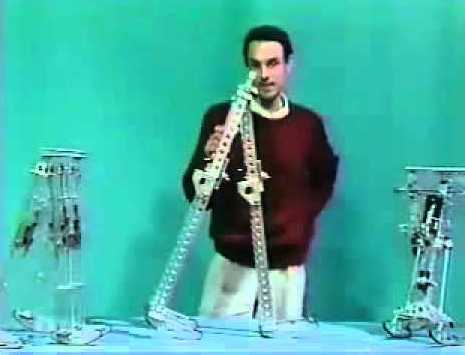
\includegraphics[width=0.49\linewidth]{tad_mcgeer.jpg}}
    \hfil
    \subfloat[][One of the Theo Jansen's creature "living" on the beach]{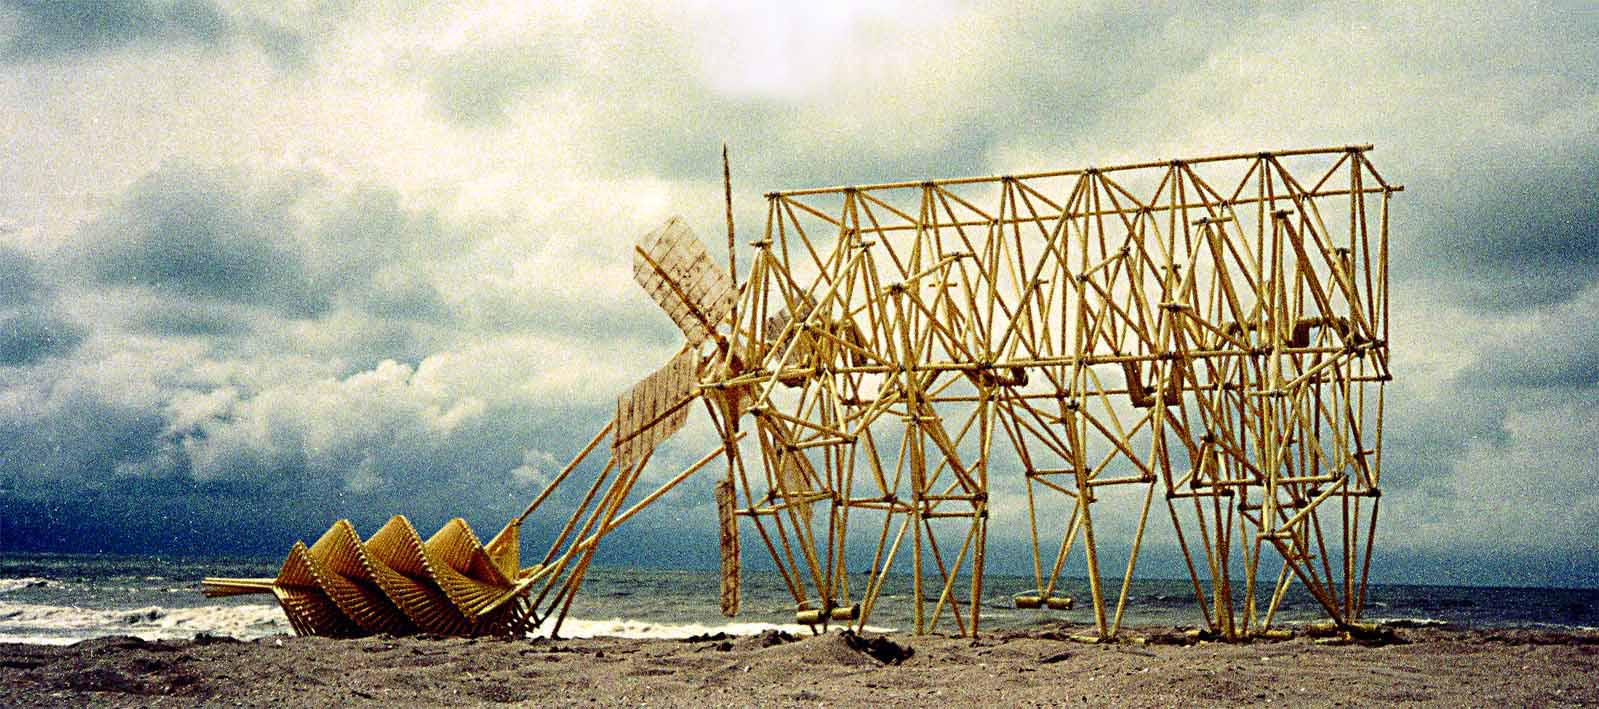
\includegraphics[width=0.99\linewidth]{theo_jansen_beast.jpg}}\newline
    \caption{}
    \label{fig:morphology_review_fr}
\end{figure}

L'un des plus célèbre est Rolf Pfeiffer qui a montré que le comportement d'un robot ne dépend pas uniquement de son contrôle mais qu'il est aussi necessaire d'integrer la morphologie du robot~\parencite{pfeifer2005morphological}. Un autre exemple très impressionnant est le travail de Tad McGeer sur de la marche passive~\parencite{mcgeer1992principles}. Son "robot" est en fait une structure purement mécanique, sans moteur, ni controlleurs. Pourtant, cette structure est capable de démontrer un comportement de marche dont la dynamique parait très similaire à celle que l'on peut observer chez l'homme. Ce comportement est uniquement le résultat des propriétés physiques de la plate-forme qui sont la longueur des segments, la forme des pieds, la position des centres de masses en interaction avec l'environnement, constitué de la gravité et d'un plan legèrement incliné. Ces travaux ont été repris plus recemment mais en conservant le même principe des chercheurs de XXX ont réussi à faire marcher un robot passif sur un tapis roulant pendant plus d'un demi heure. Un dernier exemple que l'on peut partager dans ce résumé est celui de l'artiste Theo Jansen~\parencite{jansen2007theo}. Il pratique la sculpture cinématique et son travail s'intéresse à la création de nouvelles forme de vie artificielles qui seraient capables de "vivre" de façon autonome sur les plages des Pays Bas. Il a créé un mécanisme assez original uniquement composé de tube en plastique et qui ne necessite qu'un degré de liberté faisant se mouvoir toutes les jambes en même temps. Ce mécanisme tire son energie du vent. Il a poussé ensuite le concept jusqu'à inclure des mecanismes permettant à sa structure de changer de direction, stocker l'énergie et detecter la presence d'eau. Tous ces mecanismes sont purement mécaniques et le comportement né de leurs interactions avec l'environnement.


Ces travaux montrent que le comportement d'un robot ne dépend pas uniquement du contrôle mais aussi fortement de ses propriétés morphologiques et de l'environnement dans lequel il agit.

\subsection*{Le problème de la reproductibilité}

Cependant une limite dans la pratique scientifique de ces travaux, et plus généralement en robotique, est la reproductibilité des résultats qui dépendent  fortement, comme nous l'avons vu, de la plate-forme et de sa morphologie. Ces plate-formes robotiques ne sont quasiment jamais diffusées avec les papiers scientifiques, souvent car elles sont de part leurs conception, trop difficile ou couteuse à reconstruire.

Il est alors impossible de reproduire les résultas. Pourtant lorsque l'on s'interesse à l'étude du rôle de l'incarnation et des propriétés morphologiques sur la cognition et le comportement dynamique d'un robot, la plate-forme robotique réelle avec des propriétés physiques identifiés et identiques est absolument necessaire.

\subsection*{Les plate-formes robotiques}
\label{sub:Les plate-formes robotiques}

Parmi les travaux existants, certains prototypes paraissent très interessant pour cet usage mais la plupart ne sont malheuresement pas reproductibles: leurs plans de conception n'est pas distribué et leurs morphologies sont souvent complexes avec des propriétés difficiles à reproduire.

Si l'on veut des plate-formes qui soient reproductibles dans plusieurs laboratoires, il n'y a actuellement que des plate-formes commerciales qui sont conçues pour la production en série. Elles sont par consequent reproductible, cependant leurs conception et les moyens de productions (usinage multi-axe, injection plastique,..) ne sont pas adaptée l'exploration de la morphologie car une modification de leurs structures est dans la pratique impossible (trop complexe ou couteux).

Il donc necessaire de trouver des méthodes alternatives qui permettent à la fois de considérer le corps robotique comme une variable experimentale dans lequel on peut modifier tous les parametres morphologiques. Et en même temps créer des plate-formes qui soient reproductibles dans d'autres laboratoires.

Quelques initiatives vont dans ce sens. On peut citer Locokit qui proposent des élements basiques que l'on peut assembler pour réaliser des structures mobiles dans lesquelles on peut modifier certains paramètres comme la longueur des segments ou la position des centres de masses.
Une des plate-formes les plus connues et utilisées est Icub qui a l'avantage d'avoir été reproduit en plusieurs exemplaire, d'être partagé entre different laboratoires permettant la reproduction de certaines experiences dans plusieurs laboratoires. De plus, comme cette plate-forme est open source, on pourrait en soit, modifier l'integralité du robot pour explorer differentes morphologies. Cependant les méthodes de conceptions de cette plate-forme rendent complexes et couteux sa modification. En pratique, aucun labo n'a modifié la strucutre de ce robot et seul le laboratoire d'origine travaille sur l'évolution mécanique de l'iCub.


Nous avons donc décidé de lancer le projet Poppy qui a pour but la création d'une plate-forme robotique modulaire, accessible, reproductible et communautaire.

\section*{Le projet Poppy}
\label{sec:Le projet Poppy}


Pour cela nous avons modularisé les differentes dimensions technologiques de la robotique (mécanique, electronique, informatique, ...) de telle sorte qu'elles puissent être reconfigués.

Chacun de ces modules peut être personnalisé et sont tous conçus à partir de technologie robuste, moderne, fiable et surtout facilement reproductible.

De plus, la robotique étant un domaine multi-disciplinaire, il est difficile d'être techniquement competent dans tous les domaines, nous avons donc fait en sorte que chacun des modules technologiques soit simple à prendre en main.

Creation d'une communauté robotique pour assure l'entreaide, la diffusion et surtout le developpement collaboratif.


\subsection*{Architecture Poppy}

\begin{description}
  \item[Structure mécanique]: Nous utilisons exclusivement l'impression 3D (technique de production numérique par ajout de matière) qui offre plusieurs avantages pour nos applications, en particulier son faible coût pour la production unitaire, sa rapidité, son accessibilité à tous (imprimante low cost ou sous traitance) et surtout c'est une technique reproductible car numérique, il n'y a pas besoin d'avoir de compétence particulière pour produire les pièces. Au délà des aspects pratiques, l'impression 3D permet de produire avec differents materiaux et ouvre de nouvelle possibilité en terme de design car il est possible de produire des formes qui étaient impossibles avec les techniques de production classiques.

  \item[Senseurs] Avec l'électronique, nous n'avons pas la même liberté de production rapide, low cost et unitaire. Nous avons choisis d'utiliser l'environement Arduino, ainsi toute l'acquisition des senseurs des robots Poppy est fait en utilisant des cartes Arduino (ou compatible). Elles offrent beaucoup d'entrées/sorties (numériques, analogique, bus de communication série) associées à un environnement de programmation très simple qui permet, sans aucune connaissance bas niveau sur les architecture de micro-controller de facilement interargir avec des composants electroniques.
  De plus c'est un projet open source qui a 10 ans, il y aune grosse communauté et beaucoup de developpements ont été fait, donnant accès à un grand catalogue de capteur low-cost prêt à utiliser.

  \begin{figure}[h]
      \begin{center}
          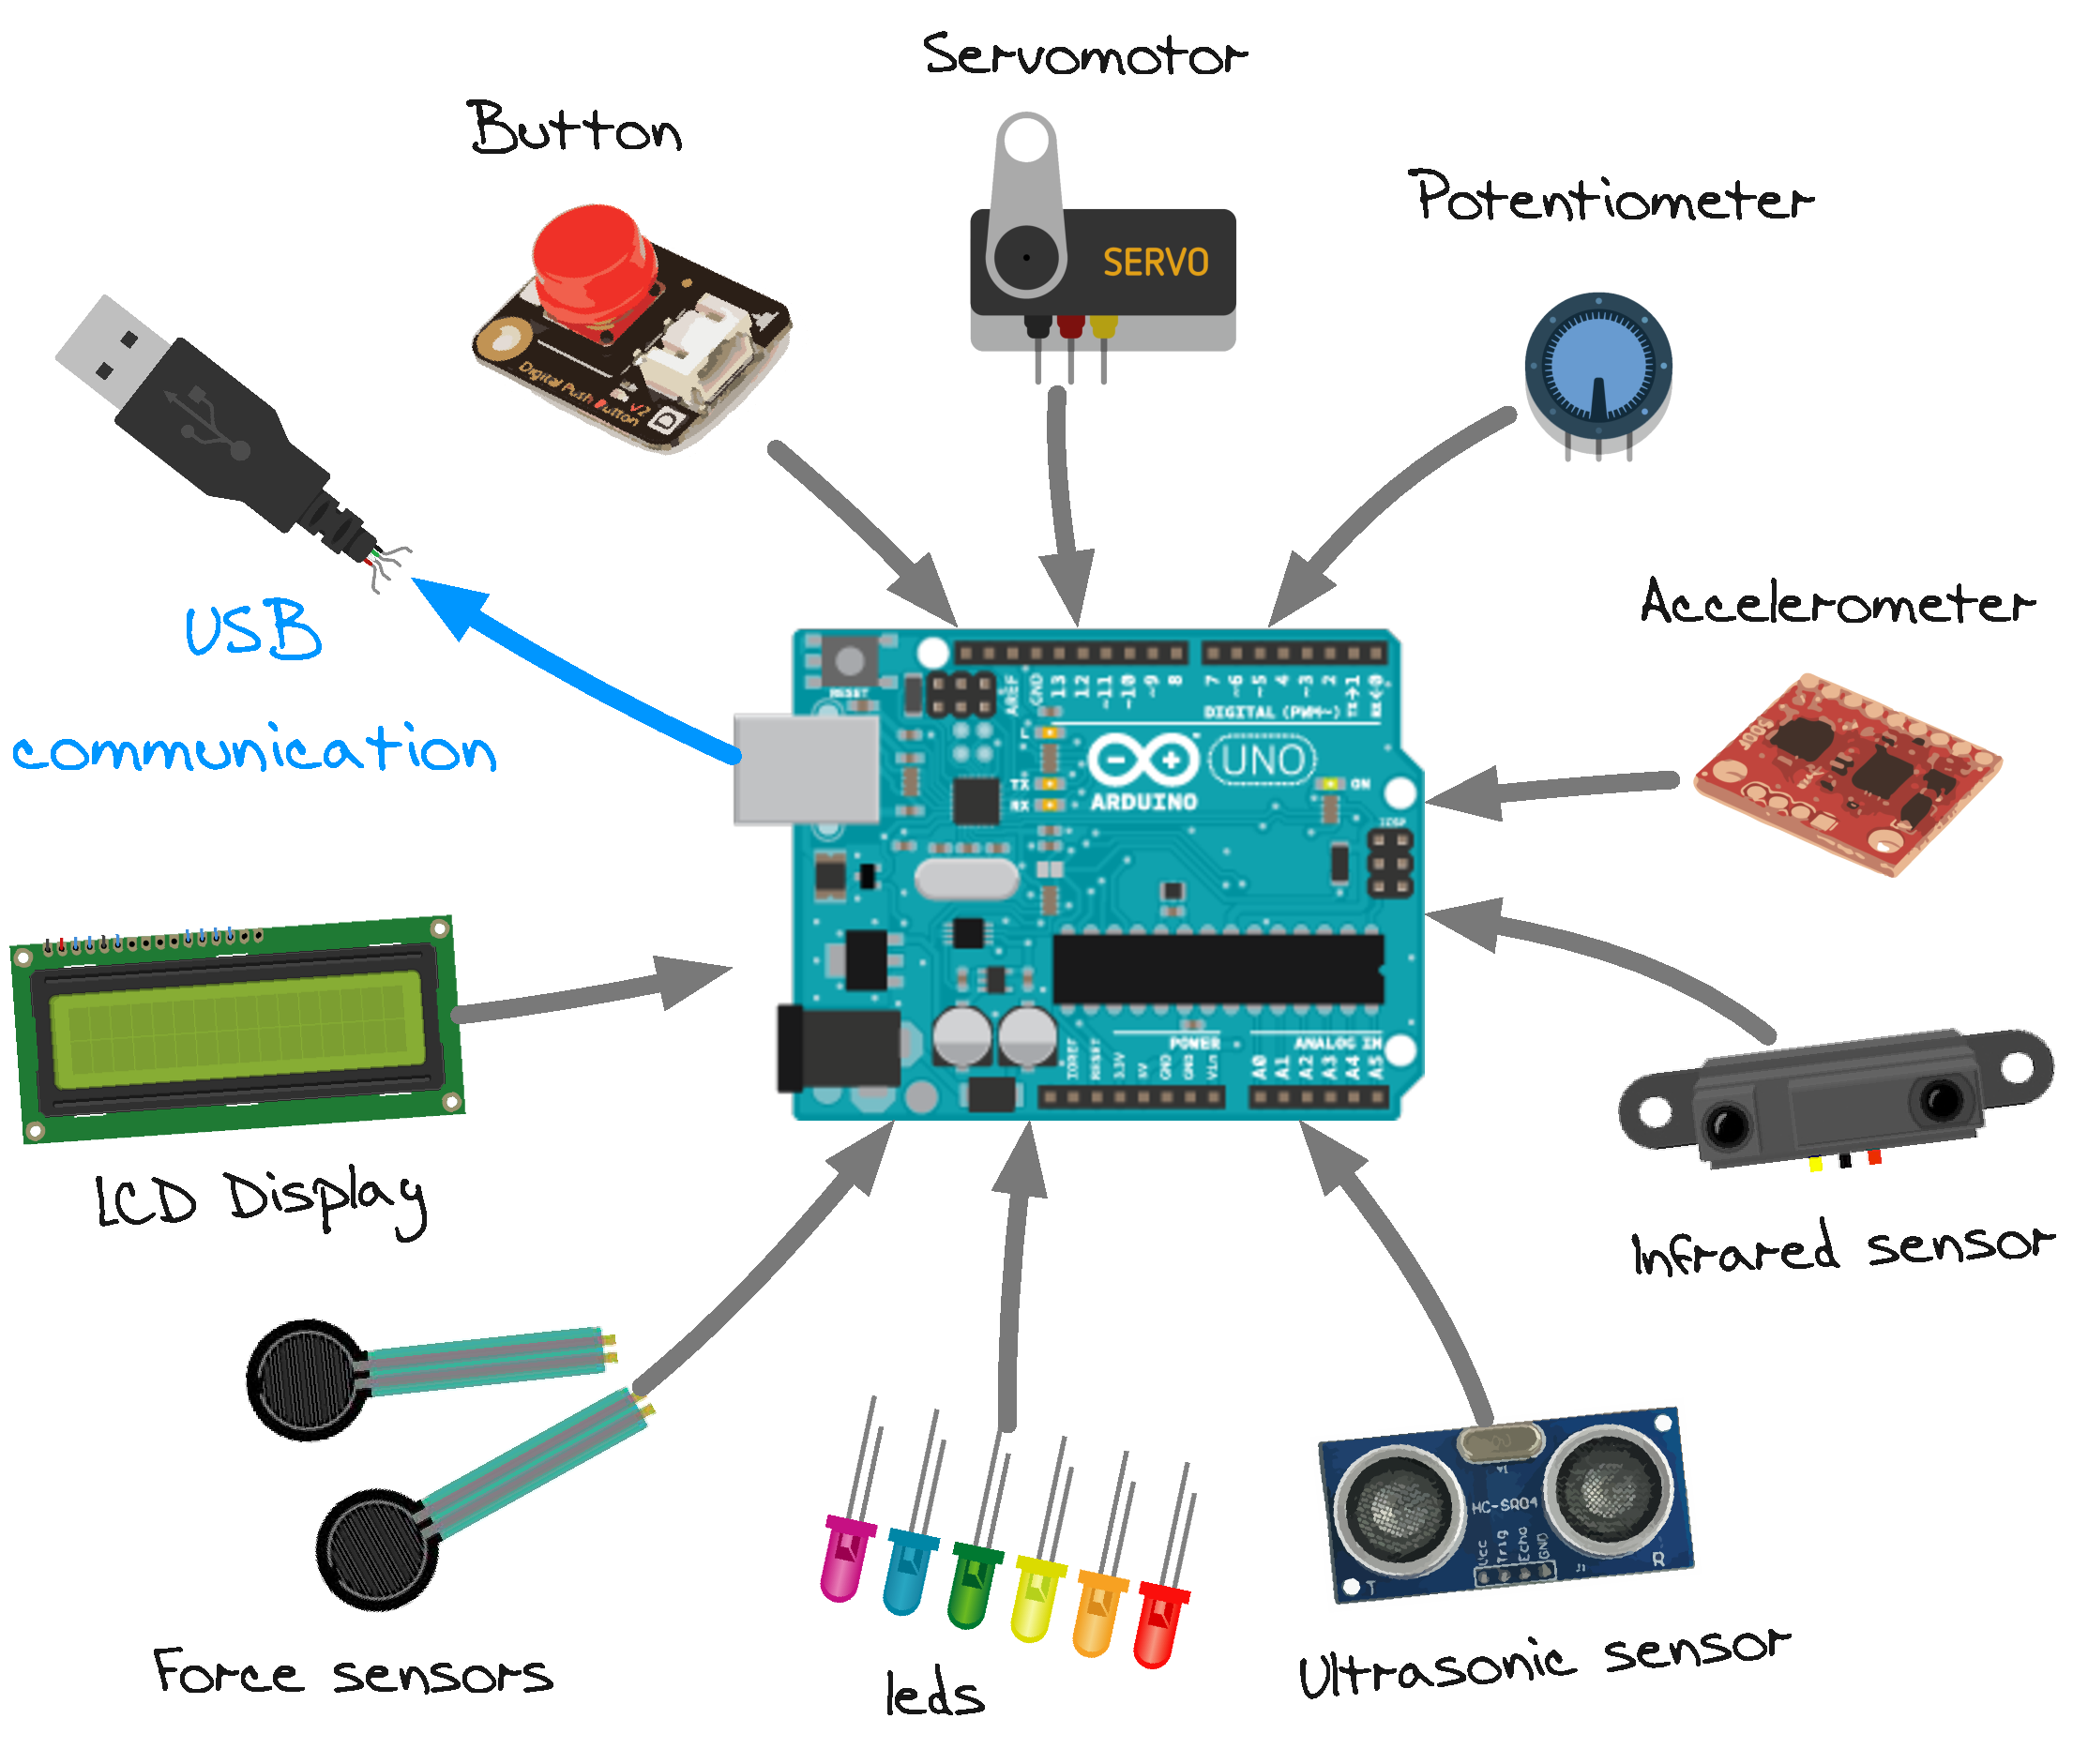
\includegraphics[width=0.9\linewidth]{arduino_electronique.pdf}
      \end{center}
      \caption{The use of Arduino as electronic architecture  allows for sensors to be easily added and/or changed, while keeping the same electronic board. In addition, it permits to add expressive components such as LEDs, LCD or sound systems, allowing users to easily explore human-robot interaction.}
      \label{fig:arduino_modular_electronic}
  \end{figure}

  Ainsi, il devient possible d'explorer assez librement differentes types et emplacements de senseurs pour modifier la morphologie d'un robot.

  \item[Actionneurs] Pour la motorisation, nous avons decidé d'utiliser les actuateurs Robotis Dynamixels car ils se présentent sous la forme d'un module tout-en-un de differentes puissances qui inclu une mécanique de qualité (moteur Maxon et engrennages en métal) ainsi qu'une carte electronique assurant le contrôle bas niveau et la mise en réseau via un bus qui permet de brancher tous les actuateurs en série. Ces modules permettent de réduire la complexité de l'assemblage et le nombre de fils.

  De plus, il est possible d'ajuster dynamiquement leurs compliance, ce qui permet l'exploration de mouvements souples ou passifs.

  \item[Contrôle] Nous avons créé une nouvelle bibliothèque de contrôle en python open source nommée pypot, 
  \item[Communauté]
\end{description}
